
\section{Structure of Nash Equilibria}

\begin{lemma}
\label{lemma:alpha_beta_independence}
Whether or not a node will switch its state is independent of the parameters $\alpha$ and $\beta$, when C=0.

\begin{proof}
From definition, we find that,
$$N(i, \mathbf{x}, 1-x_i) = N(i) - N(i, \mathbf{x}, x_i)$$
or, $$|N(i, \mathbf{x}, 1-x_i)| = |N(i) - N(i, \mathbf{x}, x_i)|$$
or, 
\begin{equation}
\label{eq:state_subtract}
|N(i, \mathbf{x}, 1-x_i)| = |N(i)| - |N(i, \mathbf{x}, x_i)|
\end{equation}

Combining Eqn.~\ref{eq:util_normal} and Eqn.~\ref{eq:state_subtract}, we get,
$$
\util(i, \mathbf{x})=\alpha|N(i, \mathbf{x}, x_i)| - \beta (|N(i)| - |N(i, \mathbf{x}, x_i)|)
$$
or,
\begin{equation}
\label{eq:util_single_param}
\util(i, \mathbf{x})= (\alpha + \beta) |N(i, \mathbf{x}, x_i)| - \beta |N(i)|
\end{equation}\\
Now, suppose, node $i$ will switch its state after time $t$.
From the \textbf{Rule} of the game, we have,
$$x_i(t+1) = 1-x(t)$$
$$\Longleftrightarrow \util(i, \mathbf{x(t)}, 1-x_i) > \util(i, \mathbf{x(t)}, x_i)$$\\
From, Eqn.~\ref{eq:util_single_param}, we have,

\begin{align}
    \Longleftrightarrow (\alpha + \beta) |N(i, \mathbf{x}, 1-x_i)| - \beta |N(i)| &> (\alpha + \beta) |N(i, \mathbf{x}, x_i)| - \beta |N(i)|\\
    \Longleftrightarrow |N(i, \mathbf{x}, 1-x_i)| &>  |N(i, \mathbf{x}, x_i)|
\label{eq:switch_condition}
\end{align}

Similarly, node $i$ will stay in the same state $x_i$.
$$x_i(t+1) = x(t)$$
$$\Longleftrightarrow \util(i, \mathbf{x(t)}, x_i) \geq \util(i, \mathbf{x(t)}, 1-x_i)$$

From, Eqn.~\ref{eq:util_single_param}, we have,

\begin{align}
    \Longleftrightarrow (\alpha + \beta) |N(i, \mathbf{x}, x_i)| - \beta |N(i)| & \geq (\alpha + \beta) |N(i, \mathbf{x}, 1-x_i)| - \beta |N(i)|\\
    \Longleftrightarrow |N(i, \mathbf{x}, 1-x_i)| & \geq  |N(i, \mathbf{x}, x_i)|
\label{eq:stay_condition}
\end{align}

Eqn.~\ref{eq:switch_condition} and  Eqn.~\ref{eq:stay_condition} are independent of  $\alpha$ and $\beta$, which completes the proof.
\end{proof}
\end{lemma}





\begin{lemma}
For every maximal strong community $S$, the state vector $\mathbf{x}$ with $x_v=1$ for all $v\in S$ and with $x_v=0$ for all $v\notin S$ is a NE.

\begin{proof}
We will use proof by contradiction.

Suppose, there is a node $A$, which belongs to a maximal strong community S and the state vector is $\mathbf{x}$ where $x_v = 1, \forall{v \in S}$.


By this assumption, $x_A = 1$.

\begin{figure}[H]
    \centering
    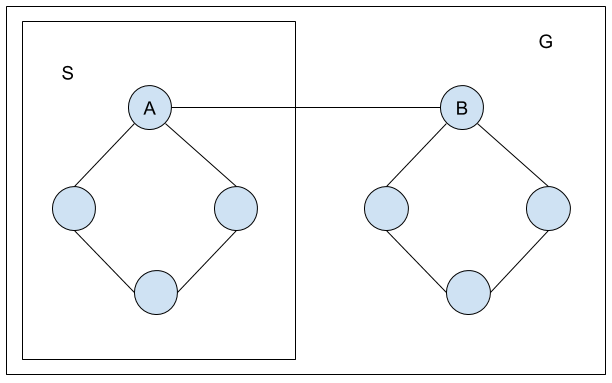
\includegraphics[width=10cm]{figs/strong_community.png}
    \caption{A Strong Community S within Graph G}
    \label{fig:strong_community}
\end{figure}

% Now, From the utility function, we can see that $A$ will switch its state if 
% \begin{align}
% \util(A, \mathbf{x}) & < 0 \\
% or, \alpha|N(A, \mathbf{x}, x_A)|  &- \beta|N(A, \mathbf{x}, 1-x_A)|  < 0 \\
% or, \alpha|N(A, \mathbf{x}, 1)|  &< \beta|N(A, \mathbf{x},0)|
% \end{align}

Now, from Lemma~\ref{lemma:alpha_beta_independence}, we have, $A$ will switch its state iff
\begin{align}
\label{eq:switch_A}
|N(A, \mathbf{x}, 1)|  < |N(A, \mathbf{x},0)|
\end{align}
\\
Now, $x_v=1, \forall{v \in S} $, which means that $x_v=1, \forall{v \in N(A) \cap S} $ \\
So, 
\begin{equation}
|N(A, \mathbf{x}, 1)| \geq |N(A) \cap S|
\end{equation}
\\
\textbf{Def.} Now, let's define $N_s(i, \mathbf{x}, x_i)$ to be the set of $i$'s of neighbors in strong community $S$ whose state is $x_i$.
\\
\\
\textbf{Def.} Similarly, let's define $N_{\bar{s}}(i, \mathbf{x}, x_i)$ to be the set of $i$'s of neighbors in $\bar{S} = G-S$ (i.e., outside the strong community $S$) whose state is $x_i$.


\begin{align}
|N(A, \mathbf{x},0)|  &= |N_s(A, \mathbf{x}, 0)| + |N_{\bar{s}}(A, \mathbf{x}, 0)|\\
& = 0 + |N_{\bar{s}}(A, \mathbf{x}, 0)|\\
& = |N_{\bar{s}}(A, \mathbf{x}, 0)|
\end{align}


Since, $N_{\bar{s}}(A, \mathbf{x}, 0) \leq|N(A) - S|$, from Eqn.~\ref{eq:switch_A}, we have,

\begin{align}
     |N(A) \cap S| < |N(A)- S|
\end{align}
% Assuming $\alpha = \beta$, we get,
% $$
% |N(A) \cap S| < |N(A)- S|
% $$
This means $A$ does not belong to the strong community, which is a contradiction.
\\
Thus, we have proved that there can be no node $A$ in $S$ which is better off by switching it's state.
\\
\\
Now, let $B$ be a node outside of the strong community $S$ which is better of by switching its state. 


Now, $x_v=1$ for all $v\in S$ and $x_v=0, \forall{v \notin S} $, which means that,
\
\begin{equation}
|N(B) - S| = |N(B, \mathbf{x}, 0)|
\end{equation}

And,
\begin{equation}
|N(B) \cap S| = |N(B, \mathbf{x}, 1)|
\end{equation}

And also, $x_B = 0$.

Now, from Lemma~\ref{lemma:alpha_beta_independence}, we have, $B$ will switch its state iff
\begin{align}
\label{eq:switch_B}
|N(B, \mathbf{x}, 1)|  > |N(B, \mathbf{x}, 0)|
\end{align}

Or.
\begin{equation}
|N(B) \cap S| > |N(B) - S|
\end{equation}

Which means that $B$ belongs to the strong community $S$, which is a contradiction. This proves that there can be no node $B \notin S$ which is better off by switching its state.
\\
\\
Combining these, we have proved that no node $A \in S$ will switch its state and no node $B \notin S$ will switch its state. Therefore, $\mathbf{x}$ is a Nash Equilibrium. 
\end{proof}

\end{lemma}

% \noindent
% \textbf{Remark.} From Eqn. (8) we see that Lemma 1 holds whenever 

% \begin{align}
    
% \end{align}
% \beta |N(A) \cap S| \geq \alpha |N(A)- S|
% $$

% \noindent
% \textbf{Structure when $\alpha\neq\beta$.}





\algdef{SE}[DOWHILE]{Do}{doWhile}{\algorithmicdo}[1]{\algorithmicwhile\ #1}

\begin{algorithm} [H]
\small{}
\caption{Sequential Best Response}\label{algo:seq-best-response}
\begin{algorithmic}[1]
    \Procedure{Sequential-Best-Response}{initial-strategy-vector}
\State $\mathbf{x}(0) \gets$ initial strategy vector
\State $|V| \gets$ len($\mathbf{x}$)
\State $\mathbf{x}(|V|) \gets$ Round1($\mathbf{x}(0)$)
\State $\mathbf{x}(2|V|) \gets$ Round2($\mathbf{x}(|V|)$)
\State \textbf{return} $\mathbf{x}(2|V|)$
\EndProcedure
\\
\\
\Procedure{Round1}{state-vector}

\State $\mathbf{x}(0) \gets$ state-vector
\State $|V| \gets$ len($\mathbf{x}$)
\For { $t \gets$ 0 to $|V|-1$}
    \State $\mathbf{x}(t+1) \gets \mathbf{x}(t) $
    
    \For{all $i \in V$ such that $x_i(t) ==  0$}
		\If{$util ( i, \mathbf{x}_{-i}(t), 1 )  >  util  ( i, \mathbf{x}_{-i}(t), 0 )$}
			\State $x_{i}(t+1) \gets 1 $
		\EndIf
\EndFor
\EndFor
\State \textbf{return} $\mathbf{x}(|V|)$
\EndProcedure
\\
\\
\Procedure{Round2}{state-vector}

\State $\mathbf{x}(0) \gets$ state-vector
\State $|V| \gets$ len($\mathbf{x}$)
\For { $t \gets$ 0 to $|V|-1$}
    \State $\mathbf{x}(t+1) \gets \mathbf{x}(t) $
    
    \For{all $i \in V$ such that $x_i(t) ==  1$}
		\If{$util ( i, \mathbf{x}_{-i}(t), 0 )  >  util  ( i, \mathbf{x}_{-i}(t), 1 )$}
			\State $x_{i}(t+1) \gets 0 $
		\EndIf
\EndFor
\EndFor
\State \textbf{return} $\mathbf{x}(|V|)$
\EndProcedure
\end{algorithmic}
\end{algorithm}
%%%%%%%%%%%%%%%%%%%%%%%%%%%%%%%%%%%%%%%%%%%%%





\begin{lemma}
The state vector $\mathbf{x}$ after Sequential Best Response is a Nash Equilibrium.

\begin{proof}
We will prove this by considering the following two cases.

\noindent
\textbf{Case 1:} Any node i in state 0 will not switch state after Round 2

At most |V| nodes can switch from 0 to 1.

At any iteration, if no node switches states: we reach NE.

So, at least 1 node must switch state in every iteration until NE.

|V| iterations are sufficient.

\noindent
\textbf{Case 2:}  Any node i in state 1 will not switch state after Round 2


There are 2 possibilities:

(a) Node i was in state 1 and didn’t switch in Round 1.

(b) Node i was in state 0 and switched in Round 2.


For both (a) and (b):

Number of nodes in state 0 can only decrease or remain unchanged after Round 2.

Utility cannot increase by switching.

\end{proof}
\end{lemma}


\begin{lemma}
Determining whether or not there exists a Nash Equilibrium with exactly K nodes in state 1 (anti-vaccine) is an NP-Hard problem.

\begin{proof}
We will prove this by reducing set-cover problem to this problem at hand.
\end{proof}
\end{lemma}